\documentclass{beamer}
\usepackage{lsfolien,enumitem}
\usepackage[german]{babel}
\usepackage[utf8]{inputenc}

\myfootline{Systemmodellierung und Semantic Web -- WS 20/21}{Hans-Gert Gräbe}

\newcommand{\ueberschrift}[1]{\begin{center}\bf #1\end{center}}

\title{Modellierung nachhaltiger Systeme\\ und Semantic Web\\[6pt] \Large
  Entwicklung von Systemen\\ und ihren Komponenten
  \vskip1em}

\subtitle{Vorlesung im Modul 10-202-2330\\ im Master und Lehramt Informatik\\
  sowie im Modul 10-202-2309 im Master Informatik}

\author{Prof. Dr. Hans-Gert Gräbe\\
\url{http://www.informatik.uni-leipzig.de/~graebe}}

\date{Wintersemester 2020/21}
\begin{document}

{\setbeamertemplate{footline}{}
\begin{frame}
  \titlepage
\end{frame}}

\section{Offene Systeme}
\begin{frame}{Dissipative Systeme und Fließgleichgewichte}

  Die Theorie dynamischer Systeme im Umfang, wie er in der letzten Vorlesung
  diskutiert wurde, beschreibt \emph{innere Dynamiken} von Systemen.

  Unser Begriff eines TS geht aber davon aus, dass Komponenten eines Systems
  in der Vollzugsdimension über deren (in der Beschreibungsform
  parametrisierten) Input/Output-Beziehungen vom System mit Aufgaben und
  Material versorgt werden.

  Da unser Konzept rekursiv ist, muss das für \emph{alle} Systeme
  vorausgesetzt werden, dass diese also stets von einem \emph{Stoff- und
    Energie-Durchsatz} angetrieben werden.

  Dazu das TRIZ-Gesetz der \emph{„Energieleitfähigkeit“ durch alle Teile des
    Systems}.
\end{frame}

\begin{frame}{Beispiele und Begriffe}
  Beispiele Bénardzelle, Lebewesen, Biosphäre der Erde.  Siehe \texttt{TDS.md}

  Begriffe (der Beschreibungsform!): 
  \begin{itemize}
  \item Eigenzeiten und Eigenräume
  \item Grenzzyklen, Attraktoren
  \item Fließgleichgewichte und dissipative Systeme
  \end{itemize}
\end{frame}

\begin{frame}{Diagramme aus (Holling 2001)}
  \begin{center}
    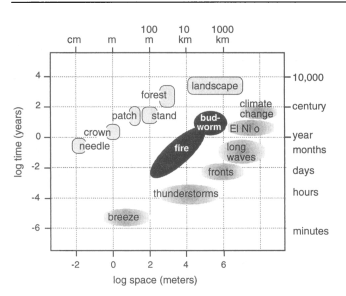
\includegraphics[width=.75\textwidth]{Holling-1.png}
  \end{center}
\end{frame}

\begin{frame}{Diagramme aus (Holling 2001)}
  \begin{center}
    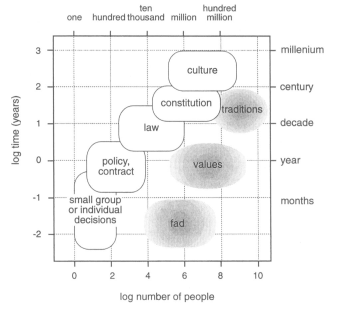
\includegraphics[width=.75\textwidth]{Holling-2.png}
  \end{center}
\end{frame}

\begin{frame}{Diagramme aus (Holling 2001)}
  \begin{center}
    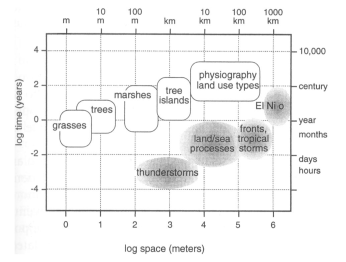
\includegraphics[width=.85\textwidth]{Holling-3.png}
  \end{center}
\end{frame}

\begin{frame}{Entwicklung von System und Komponenten}

  \emph{Beispiel:} Ein TS mit zwei Komponenten -- die Karosserieabteilung
  eines Autoherstellers mit Presserei und Lackierung.
    
  \begin{minipage}{.42\textwidth}\centering\vspace*{2em}
    \begin{tikzpicture}[line width=1pt]
        \node[draw,text width=3em, align=center] [circle] (A0) {K};
        \node[draw,below left=of A0, node distance=2em] [circle] (A1) {P};
        \node[draw,below right=of A0, node distance=2em] [circle] (A2) {L};
        \draw[-,dashed] (A0)--(A1) ;
        \draw[-,dashed] (A0)--(A2) ;
    \end{tikzpicture}\\[2em] Aufbauorganisation
  \end{minipage}\hfill
  \begin{minipage}{.55\textwidth}\centering
    \begin{tikzpicture}[line width=1pt,scale=.7,transform shape]
    \node[draw,text width=3em, align=center] [circle] (A0) {K};
    \node[draw,text width=2cm, align=center, above left=of A0] [rectangle] (I)
         {Input\\Blech}; 
    \node[draw,text width=2cm, align=center, above right=of A0] [rectangle] (O)
         {Output\\fertige\\Karosserie}; 
    \node[draw,below left=of A0, node distance=2em] [circle] (A1) {P};
    \node[draw,below right=of A0, node distance=2em] [circle] (A2) {L};
    \draw[->] (I)--(A0) ;
    \draw[->] (A0)--(O) ;
    \draw[->] (A0) to[bend right] (A1) ;
    \draw[->] (A1) to[bend right] (A0) ;
    \draw[->] (A0) to[bend right] (A2) ;
    \draw[->] (A2) to[bend right] (A0) ;
    \end{tikzpicture}\\[2em] Ablauforganisation
  \end{minipage}
\end{frame}

\begin{frame}{Entwicklung von System und Komponenten}

  \begin{minipage}{.4\textwidth}  
    \emph{Fortsetzung:} Die Presserei wird modernisiert, es werden
    Industrieroboter eingesetzt.  Wie wirkt sich das auf die „benachbarten“
    Systeme aus? Welche Szenarien sind denkbar?
  \end{minipage}\hfill
  \begin{minipage}{.55\textwidth}\centering
    \begin{tikzpicture}[scale=.55,line width=1pt,transform shape]
      \node (A0) at (0,10) {};
    \node (A4) at (3,8.5) {};
    \node (A1) at (5,7) {};
    \node (A1a) at (7,6.5) {};
    \node (A2) at (0,5) {};
    \node (A3) at (7,0) {};
    \node (A5) at (6.5,4) {};
    \node (A6) at (6,.5) {};
    \draw plot [smooth] coordinates {(A0) (A4) (A1) (A2) (A6) (A3)};
    \node[draw=red] at (4.2,9.2) [rectangle] {$r$-Phase};
    \draw[<->] (2.3,8.1) -- (3.1,7.7) ;
    \node[draw=red] at (6.2,7.5) [rectangle] {$K$-Phase};
    \draw[<->] (4.7,6.5) -- (5.5,6.5) ;
    \node[draw=red] at (8.2,6.5) [rectangle] {$\Omega$-Phase};
    \draw[->] (6.7,5.9) -- (6.6,5.3) ;
    \node[draw=red] at (8,3.8) [rectangle] {$\alpha$-Phase};
    \draw[->] (6.2,3.4) -- (6.1,2.8) ;
    \draw[<->] (5.2,.3) -- (6.2,-.2) ;
    \draw[fill=green] (A4) circle (6pt) ;
    \draw[->,dashed] plot [smooth] coordinates {(A1) (A1a) (A5) (A6)};
    \draw[fill=green] (A1) circle (6pt) ;
    \draw[fill=green] (A1a) circle (6pt) ;
    \draw[fill=green] (A5) circle (6pt) ;
    \draw[fill=green] (A6) circle (6pt) ;
    \node[draw=red,fill=white] at (7.5,0.9) [rectangle] {neue $r$-Phase};
  \end{tikzpicture}
  \end{minipage}
  
\end{frame}
\begin{frame}{Diagramme aus (Holling 2001)}
  \begin{center}
    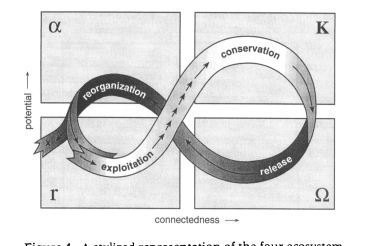
\includegraphics[width=.85\textwidth]{Holling-4.png}
  \end{center}
\end{frame}

\begin{frame}{Diagramme aus (Holling 2001)}
  \begin{center}
    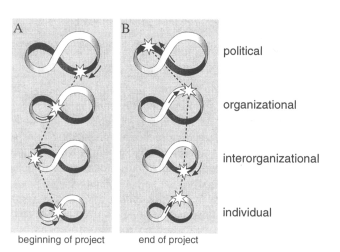
\includegraphics[width=.85\textwidth]{Holling-5.png}
  \end{center}
\end{frame}

\end{document}
